%  A simple AAU report template.
%  2015-05-08 v. 1.2.0
%  Copyright 2010-2015 by Jesper Kjær Nielsen <jkn@es.aau.dk>
%
%  This is free software: you can redistribute it and/or modify
%  it under the terms of the GNU General Public License as published by
%  the Free Software Foundation, either version 3 of the License, or
%  (at your option) any later version.
%
%  This is distributed in the hope that it will be useful,
%  but WITHOUT ANY WARRANTY; without even the implied warranty of
%  MERCHANTABILITY or FITNESS FOR A PARTICULAR PURPOSE.  See the
%  GNU General Public License for more details.
%
%  You can find the GNU General Public License at <http://www.gnu.org/licenses/>.
%
%!TEX root = ../master.tex

\documentclass[12pt,oneside,a4paper,openright, xcolor=dvipsnames]{report}




%%%%% Custom Packages and changes %%%%%
\clubpenalty = 10000
\widowpenalty = 10000
\displaywidowpenalty = 10000

\usepackage[section]{placeins}
\usepackage{pgfplots}
\usepgfplotslibrary{external} 
\pgfplotsset{compat = 1.15}
\tikzexternalize
\usepackage{adjustbox}
\usepackage{float}
\usepackage{caption}
\usepackage{subcaption}
\usepackage{upgreek}
\usepackage{fancyvrb}
\usepackage{wrapfig}
\usepackage{booktabs}

\setlength{\parindent}{0pt}

\newcommand*{\figuretitle}[1]{%
    {\centering%   <--------  will only affect the title because of the grouping (by the
    \textbf{#1}%              braces before \centering and behind \medskip). If you remove
    \par\medskip}%            these braces the whole body of a {figure} env will be centered.
}



%%%%%%%%%%%%%%%%%%%%%%%%%%%%%%%%%%%%%%%%%%%%%%%%
% Language, Encoding and Fonts
% http://en.wikibooks.org/wiki/LaTeX/Internationalization
%%%%%%%%%%%%%%%%%%%%%%%%%%%%%%%%%%%%%%%%%%%%%%%%
% Select encoding of your inputs. Depends on
% your operating system and its default input
% encoding. Typically, you should use
%   Linux  : utf8 (most modern Linux distributions)
%            latin1 
%   Windows: ansinew
%            latin1 (works in most cases)
%   Mac    : applemac
% Notice that you can manually change the input
% encoding of your files by selecting "save as"
% an select the desired input encoding. 
\usepackage[utf8]{inputenc}

% Make latex understand and use the typographic
% rules of the language used in the document.
\usepackage[german,english]{babel}
% Use the palatino font
%\usepackage[sc]{mathpazo}
%\linespread{1.05}         % Palatino needs more leading (space between lines)
% Choose the font encoding
\usepackage[T1]{fontenc}
%%%%%%%%%%%%%%%%%%%%%%%%%%%%%%%%%%%%%%%%%%%%%%%%
% Graphics and Tables
% http://en.wikibooks.org/wiki/LaTeX/Importing_Graphics
% http://en.wikibooks.org/wiki/LaTeX/Tables
% http://en.wikibooks.org/wiki/LaTeX/Colors
%%%%%%%%%%%%%%%%%%%%%%%%%%%%%%%%%%%%%%%%%%%%%%%%
% load a colour package
\usepackage{xcolor}
\definecolor{aaublue}{RGB}{33,26,82}% dark blue
% The standard graphics inclusion package
\usepackage{graphicx}
% Set up how figure and table captions are displayed
\usepackage{caption}
\captionsetup{%
  font=footnotesize,% set font size to footnotesize
  labelfont=bf % bold label (e.g., Figure 3.2) font
}
% Make the standard latex tables look so much better
\usepackage{array,booktabs}
% Enable the use of frames around, e.g., theorems
% The framed package is used in the example environment
\usepackage{framed}

%%%%%%%%%%%%%%%%%%%%%%%%%%%%%%%%%%%%%%%%%%%%%%%%
% Mathematics
% http://en.wikibooks.org/wiki/LaTeX/Mathematics
%%%%%%%%%%%%%%%%%%%%%%%%%%%%%%%%%%%%%%%%%%%%%%%%
% Defines new environments such as equation,
% align and split 
\usepackage{amsmath}
% Adds new math symbols
\usepackage{amssymb}
% Use theorems in your document
% The ntheorem package is also used for the example environment
% When using thmmarks, amsmath must be an option as well. Otherwise \eqref doesn't work anymore.
\usepackage[framed,amsmath,thmmarks]{ntheorem}

%%%%%%%%%%%%%%%%%%%%%%%%%%%%%%%%%%%%%%%%%%%%%%%%
% Page Layout
% http://en.wikibooks.org/wiki/LaTeX/Page_Layout
%%%%%%%%%%%%%%%%%%%%%%%%%%%%%%%%%%%%%%%%%%%%%%%%
% Change margins, papersize, etc of the document
\usepackage[
  left=25mm,% left margin on an odd page
  right=25mm,% right margin on an odd page
  top=25mm,
  bottom=25mm
  ]{geometry}
% Modify how \chapter, \section, etc. look
% The titlesec package is very configureable
\usepackage{titlesec}
\titleformat{\chapter}[hang]{\normalfont\LARGE\bfseries}{\ \thechapter.}{20pt}{\LARGE}
\titleformat*{\section}{\normalfont\large\bfseries}
\titleformat*{\subsection}{\normalfont\normalsize\bfseries}
\titleformat*{\subsubsection}{\normalfont\normalsize\bfseries}
%\titleformat*{\paragraph}{\normalfont\normalsize\bfseries}
%\titleformat*{\subparagraph}{\normalfont\normalsize\bfseries}

\titlespacing*{\chapter}{0pt}{*8}{*3}
\titlespacing*{\section}{0pt}{*3}{*1}
\titlespacing*{\subsection}{0pt}{*2}{*1}
\titlespacing*{\subsubsection}{0pt}{*2}{*0}

% Clear empty pages between chapters
%\let\origdoublepage\cleardoublepage
%\newcommand{\clearemptydoublepage}{%
%  \clearpage
%  {\pagestyle{empty}\origdoublepage}%
%}
%\let\cleardoublepage\clearemptydoublepage

% NO clear empty pages between chapters
    \makeatletter
    \renewcommand\chapter{\par%
       \thispagestyle{plain}%
       \global\@topnum\z@
       \@afterindentfalse
       \secdef\@chapter\@schapter}
    \makeatother

% Change the headers and footers
\usepackage{fancyhdr}
\pagestyle{fancy}
\fancyhf{} %delete everything
\renewcommand{\headrulewidth}{0pt} %remove the horizontal line in the header
\fancyhead[RO]{\small\nouppercase\rightmark} %even page - chapter title
%\fancyhead[LO]{\small\nouppercase\rightmark} %uneven page - section title
%\fancyhead[LE,RO]{\thepage} %page number on all pages
\cfoot{\thepage}
% Do not stretch the content of a page. Instead,
% insert white space at the bottom of the page
\raggedbottom
% Enable arithmetics with length. Useful when
% typesetting the layout.
\usepackage{calc}

%%%%%%%%%%%%%%%%%%%%%%%%%%%%%%%%%%%%%%%%%%%%%%%%
% Bibliography
% http://en.wikibooks.org/wiki/LaTeX/Bibliography_Management
%%%%%%%%%%%%%%%%%%%%%%%%%%%%%%%%%%%%%%%%%%%%%%%%
%\usepackage[backend=bibtex, bibencoding=utf8 ]{biblatex}
\usepackage[round,sort,authoryear]{natbib}
\bibliographystyle{unsrtnat}
%\addbibresource{bib/mybib}
%%%%%%%%%%%%%%%%%%%%%%%%%%%%%%%%%%%%%%%%%%%%%%%%
% Misc
%%%%%%%%%%%%%%%%%%%%%%%%%%%%%%%%%%%%%%%%%%%%%%%%
% Add bibliography and index to the table of
% contents
\usepackage[nottoc]{tocbibind}
% Add the command \pageref{LastPage} which refers to the
% page number of the last page
\usepackage{lastpage}
% Add todo notes in the margin of the document
\usepackage[
%  disable, %turn off todonotes
  colorinlistoftodos, %enable a coloured square in the list of todos
  textwidth=\marginparwidth, %set the width of the todonotes
  textsize=scriptsize, %size of the text in the todonotes
  ]{todonotes}

%%%%%%%%%%%%%%%%%%%%%%%%%%%%%%%%%%%%%%%%%%%%%%%%
% Hyperlinks
% http://en.wikibooks.org/wiki/LaTeX/Hyperlinks
%%%%%%%%%%%%%%%%%%%%%%%%%%%%%%%%%%%%%%%%%%%%%%%%
% Enable hyperlinks and insert info into the pdf
% file. Hypperref should be loaded as one of the 
% last packages
\usepackage{hyperref}
\hypersetup{%
	pdfpagelabels=true,%
	plainpages=false,%
	pdfauthor={Author(s)},%
	pdftitle={Title},%
	pdfsubject={Subject},%
	bookmarksnumbered=true,%
	colorlinks=false,%
	citecolor=black,%
	filecolor=black,%
	linkcolor=black,% you should probably change this to black before printing
	urlcolor=black,%
	pdfstartview=FitH%
}

% package inclusion and set up of the document
% see, e.g., http://en.wikibooks.org/wiki/LaTeX/Formatting#Hyphenation
% for more information on word hyphenation
\hyphenation{ex-am-ple hy-phen-a-tion short}
\hyphenation{long la-tex}% 
%  A simple AAU report template.
%  2015-05-08 v. 1.2.0
%  Copyright 2010-2015 by Jesper Kjær Nielsen <jkn@es.aau.dk>
%
%  This is free software: you can redistribute it and/or modify
%  it under the terms of the GNU General Public License as published by
%  the Free Software Foundation, either version 3 of the License, or
%  (at your option) any later version.
%
%  This is distributed in the hope that it will be useful,
%  but WITHOUT ANY WARRANTY; without even the implied warranty of
%  MERCHANTABILITY or FITNESS FOR A PARTICULAR PURPOSE.  See the
%  GNU General Public License for more details.
%
%  You can find the GNU General Public License at <http://www.gnu.org/licenses/>.
%
%
%
% see, e.g., http://en.wikibooks.org/wiki/LaTeX/Customizing_LaTeX#New_commands
% for more information on how to create macros

%%%%%%%%%%%%%%%%%%%%%%%%%%%%%%%%%%%%%%%%%%%%%%%%
% Macros for the titlepage
%%%%%%%%%%%%%%%%%%%%%%%%%%%%%%%%%%%%%%%%%%%%%%%%
%Creates the aau titlepage
\newcommand{\aautitlepage}[3]{%
  {
    %set up various length
    \ifx\titlepageleftcolumnwidth\undefined
      \newlength{\titlepageleftcolumnwidth}
      \newlength{\titlepagerightcolumnwidth}
    \fi
    \setlength{\titlepageleftcolumnwidth}{0.5\textwidth-\tabcolsep}
    \setlength{\titlepagerightcolumnwidth}{\textwidth-2\tabcolsep-\titlepageleftcolumnwidth}
    %create title page
    \thispagestyle{empty}
    \noindent%
    \begin{tabular}{@{}ll@{}}
      \parbox{\titlepageleftcolumnwidth}{
        \iflanguage{danish}{%
          \includegraphics[width=\titlepageleftcolumnwidth]{figures/Uni-Goettingen-Logo.pdf}
        }{%
          \includegraphics[width=\titlepageleftcolumnwidth]{figures/Uni-Goettingen-Logo.pdf}
        }
      } &
      \parbox{\titlepagerightcolumnwidth}{\raggedleft\sf\small
        #2
      }\bigskip\\ \bigskip\\ \bigskip\\
       #1 &
      
    \end{tabular}
    \vfill
    \clearpage
  }
}

%Create english project info
\newcommand{\englishprojectinfo}[8]{%
  \parbox[t]{\titlepageleftcolumnwidth}{
    \textbf{Title:}\\ #1\bigskip\par
    \textbf{Theme:}\\ #2\bigskip\par
    \textbf{Project Period:}\\ #3\bigskip\par
    \textbf{Project Group:}\\ #4\bigskip\par
    \textbf{Participant(s):}\\ #5\bigskip\par
    \textbf{Supervisor(s):}\\ #6\bigskip\par
    \textbf{Copies:} #7\bigskip\par
    \textbf{Page Numbers:} \pageref{LastPage}\bigskip\par
    \textbf{Date of Completion:}\\ #8
  }
}

%Create danish project info
\newcommand{\danishprojectinfo}[8]{%
  \parbox[t]{\titlepageleftcolumnwidth}{
    \textbf{Titel:}\\ #1\bigskip\par
    \textbf{Tema:}\\ #2\bigskip\par
    \textbf{Projektperiode:}\\ #3\bigskip\par
    \textbf{Projektgruppe:}\\ #4\bigskip\par
    \textbf{Deltager(e):}\\ #5\bigskip\par
    \textbf{Vejleder(e):}\\ #6\bigskip\par
    \textbf{Oplagstal:} #7\bigskip\par
    \textbf{Sidetal:} \pageref{LastPage}\bigskip\par
    \textbf{Afleveringsdato:}\\ #8
  }
}

%%%%%%%%%%%%%%%%%%%%%%%%%%%%%%%%%%%%%%%%%%%%%%%%
% An example environment
%%%%%%%%%%%%%%%%%%%%%%%%%%%%%%%%%%%%%%%%%%%%%%%%
\theoremheaderfont{\normalfont\bfseries}
\theorembodyfont{\normalfont}
\theoremstyle{break}
\def\theoremframecommand{{\color{gray!50}\vrule width 5pt \hspace{5pt}}}
\newshadedtheorem{exa}{Example}[chapter]
\newenvironment{example}[1]{%
		\begin{exa}[#1]
}{%
		\end{exa}
}% my new macros

\DeclareUnicodeCharacter{2212}{-}
%\DeclareUnicodeCharacter{FB00}{ff}

%\DeclareUnicodeCharacter{U+00B4}{}
%\pgfplotset
\begin{document}
%frontmatter
\pagestyle{empty} %disable headers and footers
\pagenumbering{roman} %use roman page numbering in the frontmatter
%  A simple AAU report template.
%  2015-05-08 v. 1.2.0
%  Copyright 2010-2015 by Jesper Kjær Nielsen <jkn@es.aau.dk>
%
%  This is free software: you can redistribute it and/or modify
%  it under the terms of the GNU General Public License as published by
%  the Free Software Foundation, either version 3 of the License, or
%  (at your option) any later version.
%
%  This is distributed in the hope that it will be useful,
%  but WITHOUT ANY WARRANTY; without even the implied warranty of
%  MERCHANTABILITY or FITNESS FOR A PARTICULAR PURPOSE.  See the
%  GNU General Public License for more details.
%
%  You can find the GNU General Public License at <http://www.gnu.org/licenses/>.
%
\pdfbookmark[0]{Front page}{label:frontpage}%
\begin{titlepage}
  \addtolength{\hoffset}{0.5\evensidemargin-0.5\oddsidemargin} %set equal margins on the frontpage - remove this line if you want default margins
  \noindent%
  \begin{tabular}{@{}p{\textwidth}@{}}
    \toprule[2pt]
    \midrule
    \vspace{0.2cm}
    \begin{center}
    \Huge{\textbf{
      Application Exercise
    }}
    \end{center}
    \begin{center}
      \Large{
        Nikos Bosse
      }
    \end{center}
    \vspace{0.2cm}\\
    \midrule
    \toprule[2pt]
  \end{tabular}
  \vspace{4 cm}
  \vfill
\end{titlepage}
\clearpage

%\cleardoublepage
\pdfbookmark[0]{Contents}{label:contents}
\pagestyle{fancy} %enable headers and footers again
\tableofcontents
\clearpage
%\listoftodos
%\cleardoublepage
%mainmatter
\pagenumbering{arabic} %use arabic page numbering in the mainmatter


%!TEX root = ../master.tex"`


\chapter{Proposed Trading Strategy}

In the data, almost all of profits are driven by the extremely unusual Asset2. A strategy that would have performed well would therefore have been a strategy centered on Asset2, or more general a momentum-like trading strategy that would have invested in stocks that have performed well in the past. This is of course easy to say in hindsight. Frankly, I don't think I could be very confident in recommending something other than a simple buy-and-hold strategy (maybe improved by some more elegant ways to optimally balance risks and profits in the portfolio). But then again this is why I am applying to this job: I am eager to learn more. 

There is, however, a couple of things that I have tried and some analyses I have run that are interesting in and of themselves. 

\section{General process for deriving a strategy}
\subsection{Data Preparation and Visualization}
I have split the data in training and test data set. I've done this for a couple of split dates, but present only the results for a training period of the first 1500 observations. As an initial step I extracted log returns and made sure that all time series are stationary see results \slash train\_stationarity.csv with the Augmented Dickey-Fuller test. 

Then I plotted the data. It can be seen results in Figure \ref{1} that everything is dominated by Asset2. 

\begin{figure}[h!]
    %\figuretitle{Stock Prices}
    \centering
    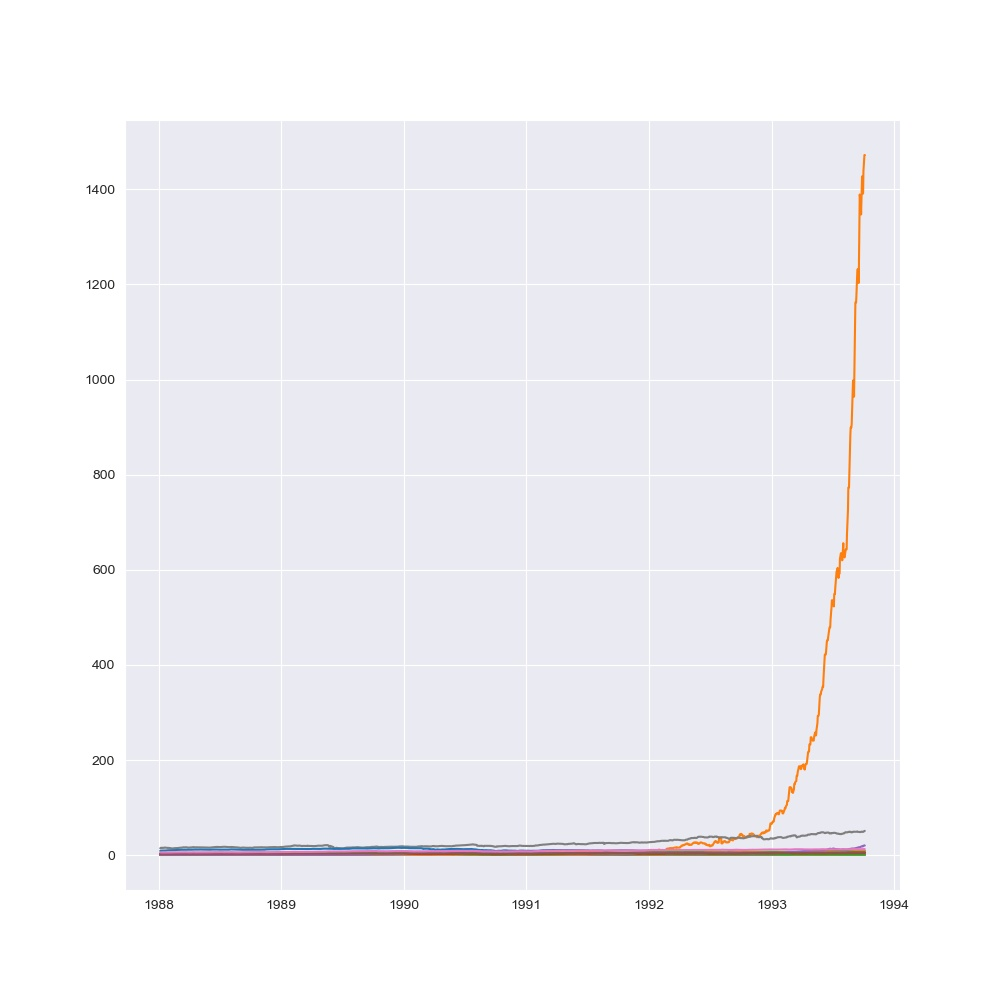
\includegraphics[width=0.48\textwidth]{../results/train_all_assets.jpg}
    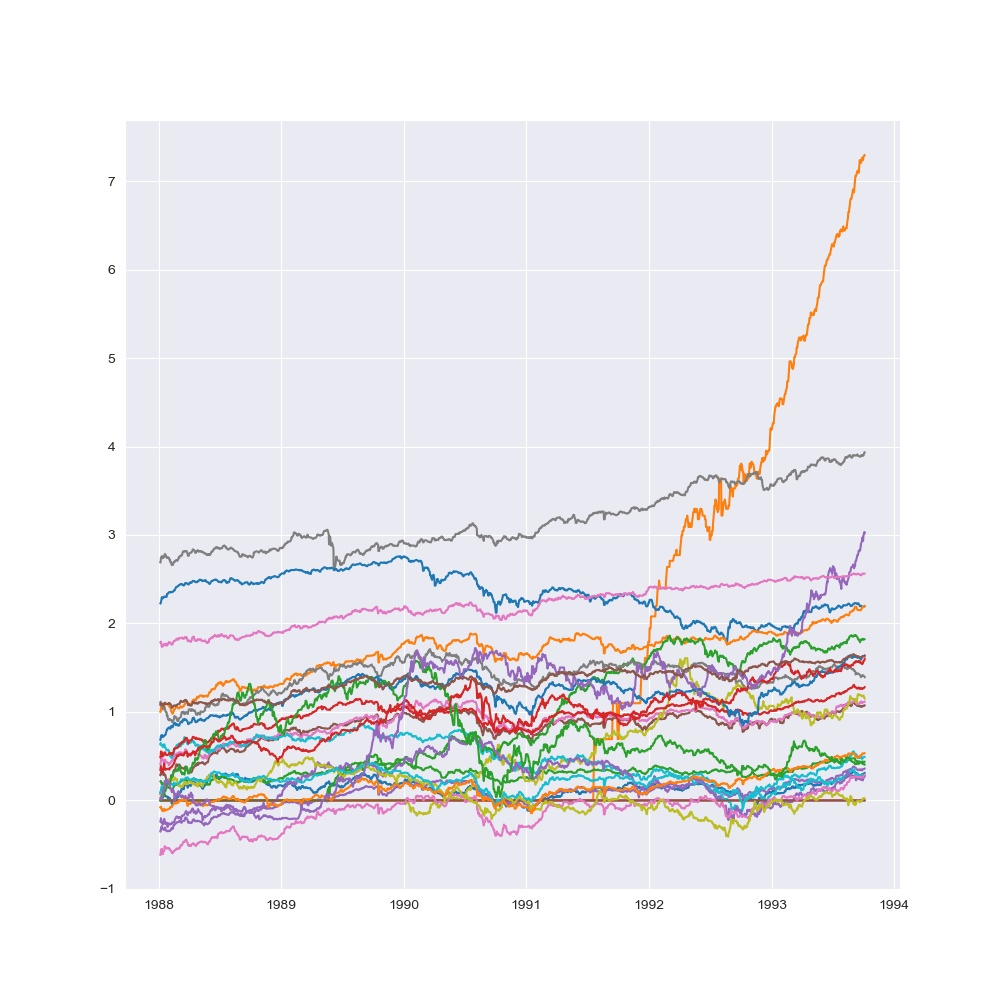
\includegraphics[width=0.48\textwidth]{../results/train_all_assets_logged.jpg}
    \caption{All Assets first 1500 obs}
    \label{1}
  
\end{figure}{}

\subsection{Look at Autocorrelations}
As can be seen in results \slash all\_autocorr\_log\_returns.jpg, log returns of the assets generally do not exhibit large amounts of autocorrelation. While it is of course possible to fit different time series models to the data I do not feel confident that I would not simply overfit to past observations. I have also looked at automatically selected arma orders (see results\slash train\_select\_arma\_order.csv). One can see that BIC values for the different orders do hardly change. I therefore have little confidence in the ARMA orders automatically chosen. I nevertheless implemented a trading strategy based on time series predictions. Right now it only looks at ARMA(1,1)-models, but it can be easily replaced by an auto-ARMA model. This trading strategy performs very poorly right now. One can adapt the threshold value in the trade-method of the python object, but I still have little confidence in this strategy and implemented it rather as a proof of principle. 


\subsection{Look at Cointegration}
Extensive literature suggests one can use cointegrated time series to construct a trading strategy that profits from the fact that time series move together. I tried all combinations of the time series and found combinations with p-values smaller than 0.05. However, none of them remained after adjusting for the testing of (sum(1, ..., 26) * 2) = 702 combinations. Also cointegration values differed greatly for different lengths of the time series. With more time, I would have liked to have a more thorough look at this. I did not implement a cointegration based strategy, because this would have meant focusing only on pairs of stocks instead of the entire portfolio. 

\subsection{Look at Conditional Heteroskedasticity}
As can be seen in results \slash train\_all\_autocorr\_squared\_log\_returns.jpg, the assets exhibit Conditional Heteroskedasticity. The squared log returns are oftentimes autocorrelated at lag 1, 5, 10 One could therefore model risks according to predicted variations in future returns. With more time, I would have looked into this to devise a trading strategy that uses this for risk management. 



\chapter{Results of the implemented trading strategies}

\section{Results for the training period}
Results are shown in Figure \ref{2}. The momentum based strategy is by far the best, however it is not able to outperform a buy-and-hold strategy. Figure \ref{3} shows a sanity check with the Assets 2 and 25 removed. Again, both mean reversion and momentum trading perform worse than the baseline. 


\begin{figure}[h!]
    %\figuretitle{Stock Prices}
    \centering
    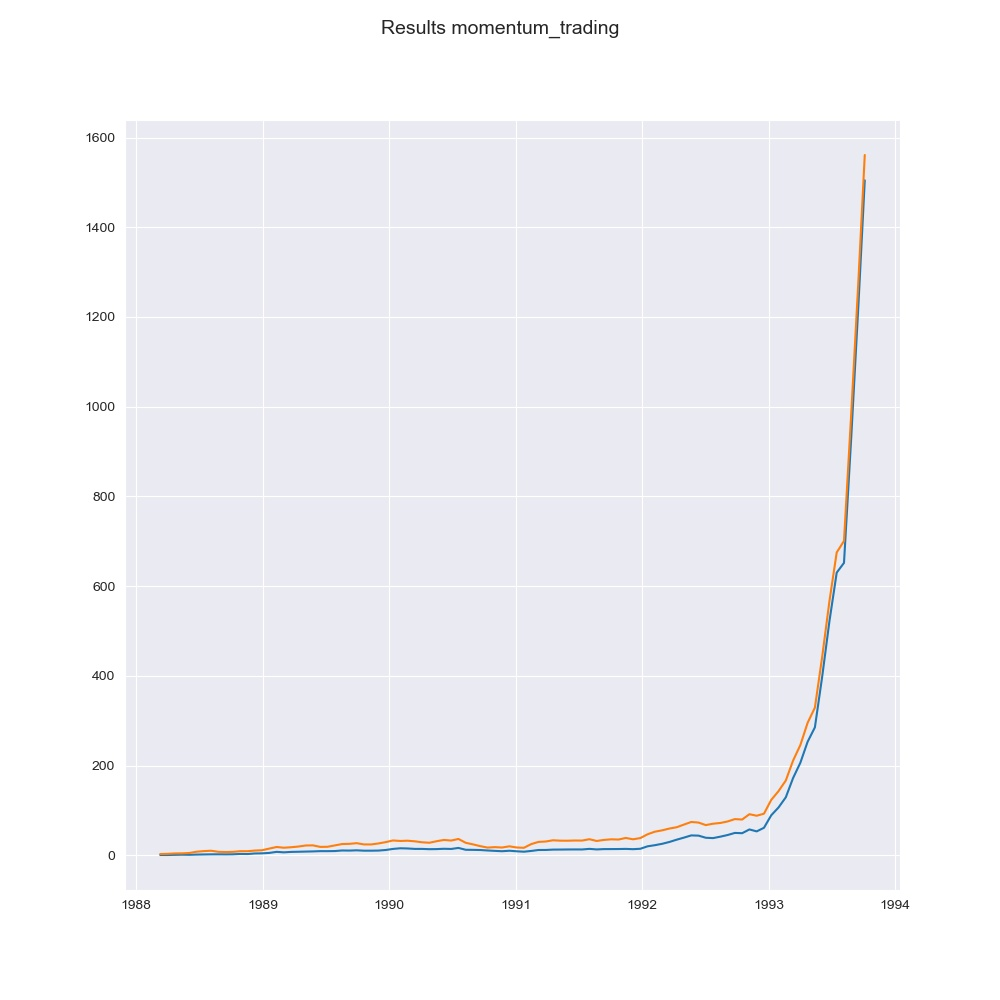
\includegraphics[width=0.48\textwidth]{../results/train_momentum_trading_results.jpg}
    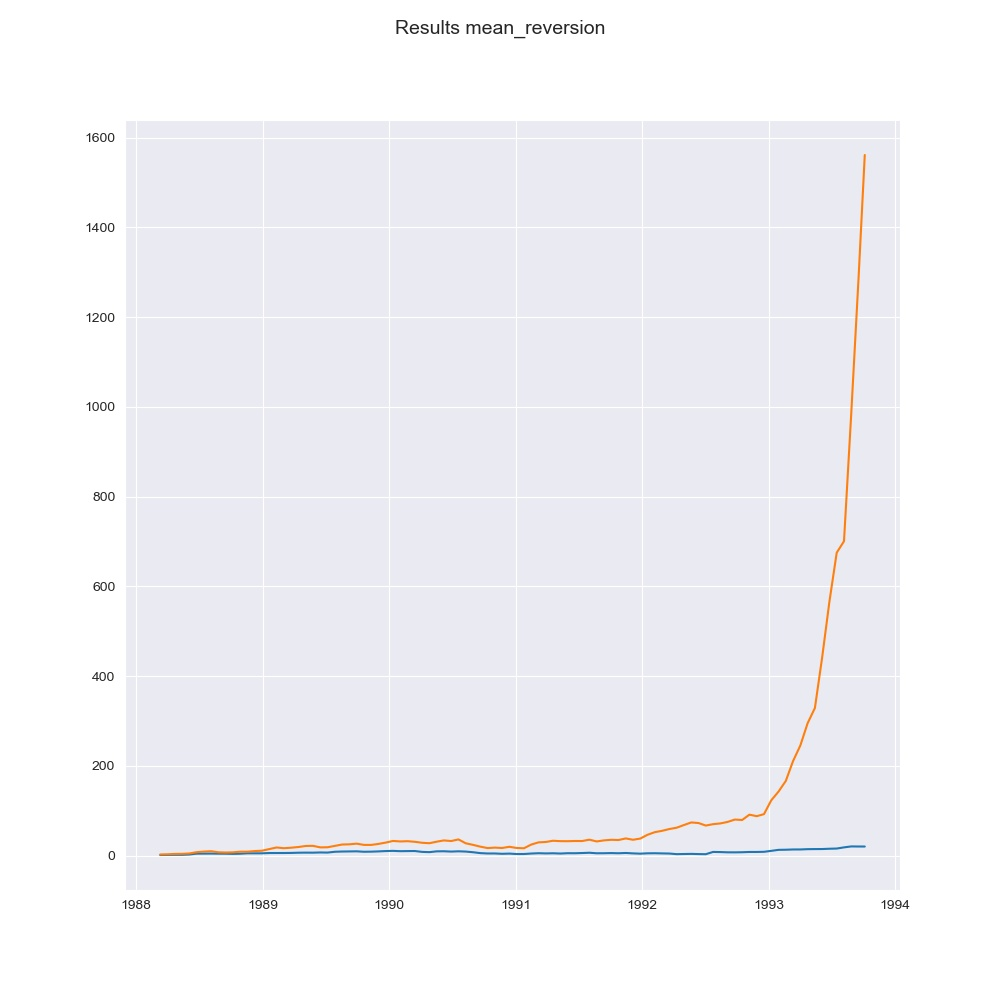
\includegraphics[width=0.48\textwidth]{../results/train_mean_reversion_results.jpg}

    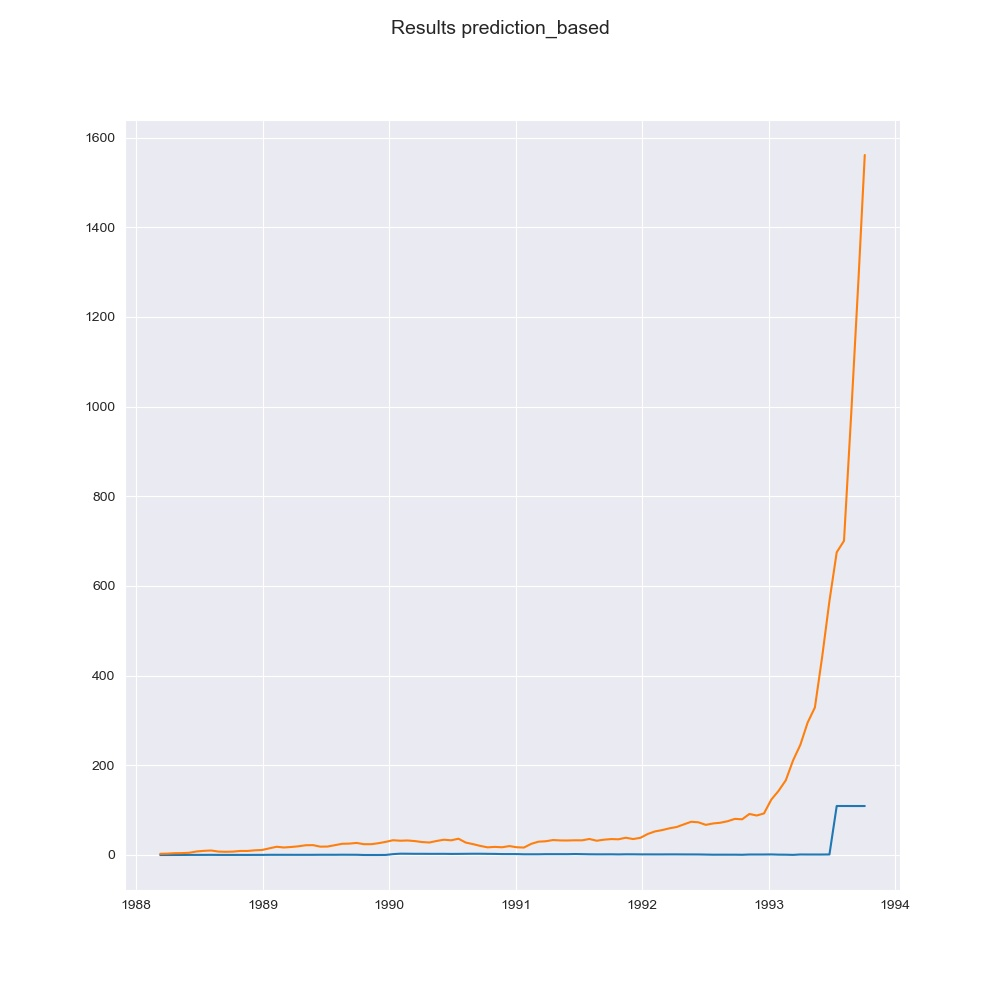
\includegraphics[width=0.48\textwidth]{../results/train_prediction_based_results.jpg}

    \caption{Results first 1500 obs, baseline in orange}
    \label{2}
  
\end{figure}{}

\begin{figure}[h!]
    %\figuretitle{Stock Prices}
    \centering
    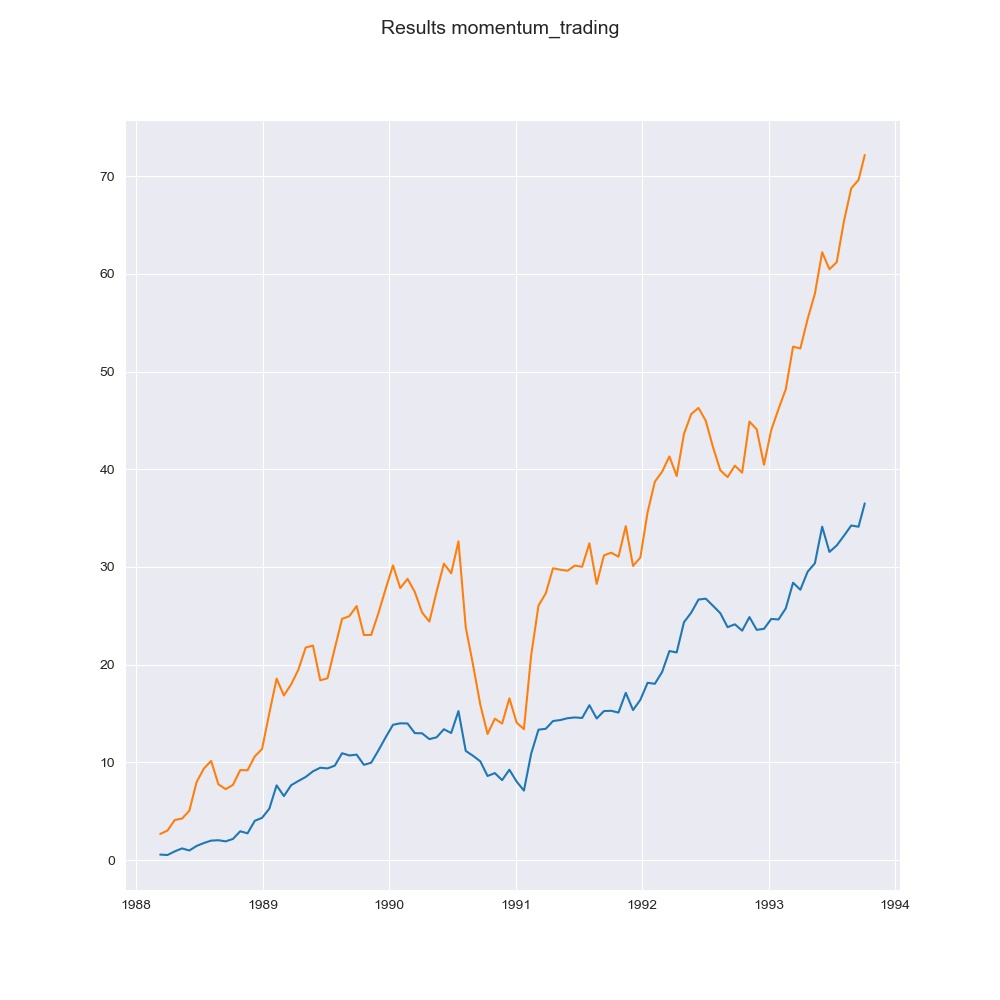
\includegraphics[width=0.48\textwidth]{../results/train_outliers_removed_momentum_trading_results.jpg}
    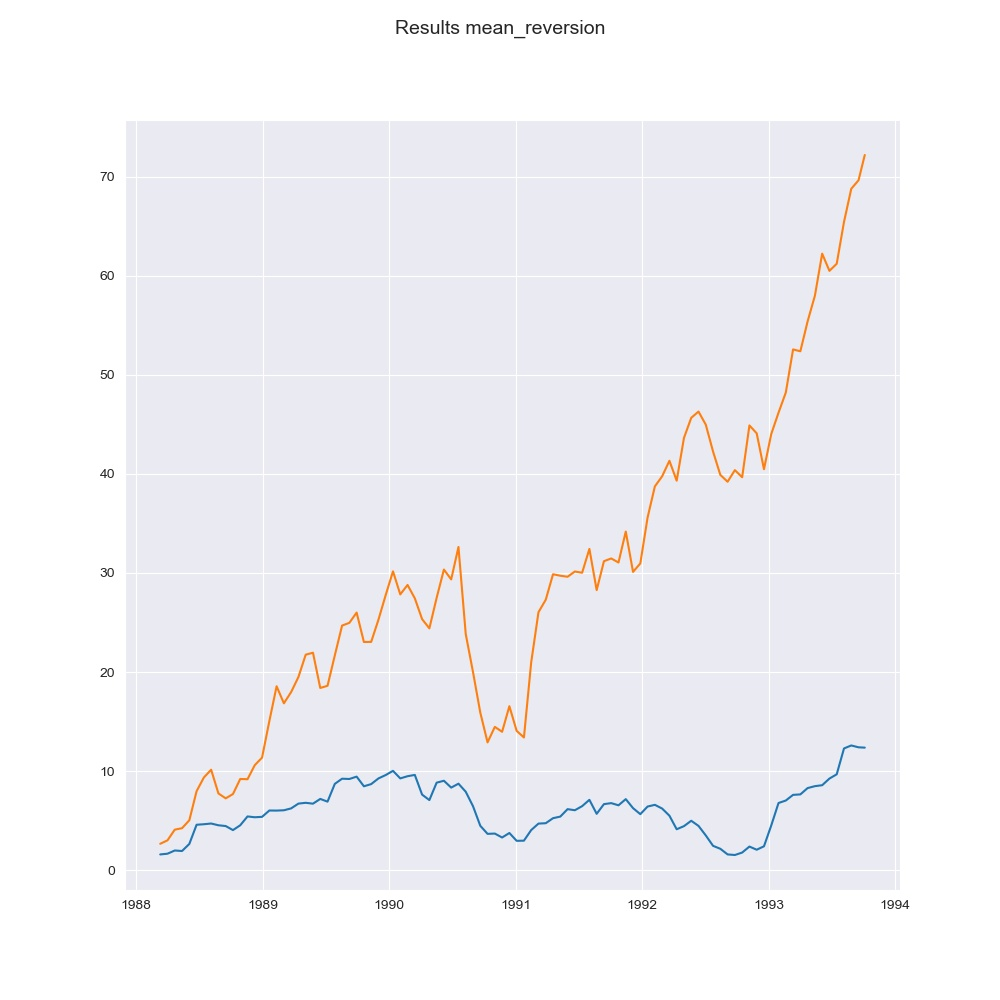
\includegraphics[width=0.48\textwidth]{../results/train_outliers_removed_mean_reversion_results.jpg}

    \caption{Results first 1500 obs, Assets 2 and 25 removed, baseline in orange}
    \label{3}
  
\end{figure}{}


\section{Results for the whole period}
Results for the whole data set are shown in Figure \ref{4}. Again, momentum trading and mean reversion perform worse than buy-and-hold. 

\begin{figure}[h!]
    %\figuretitle{Stock Prices}
    \centering
    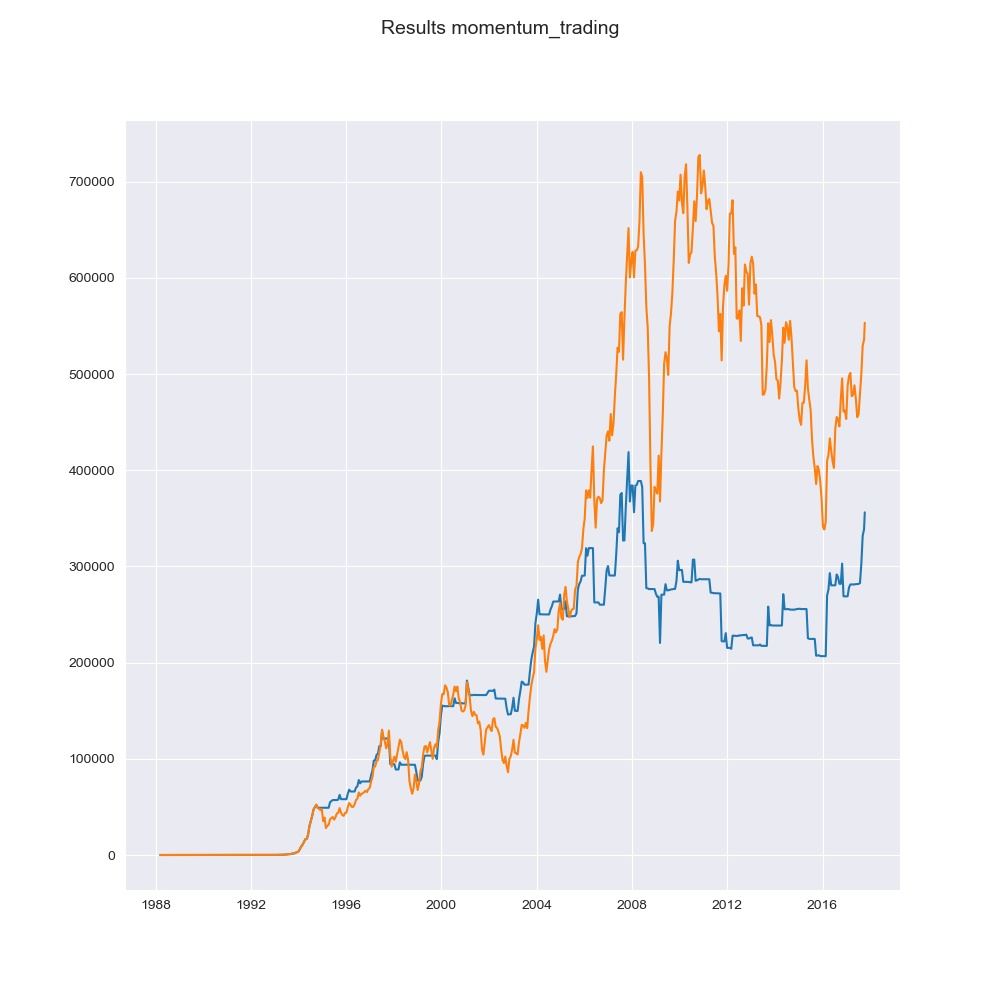
\includegraphics[width=0.48\textwidth]{../results/results_full_ts/momentum_trading_results.jpg}
    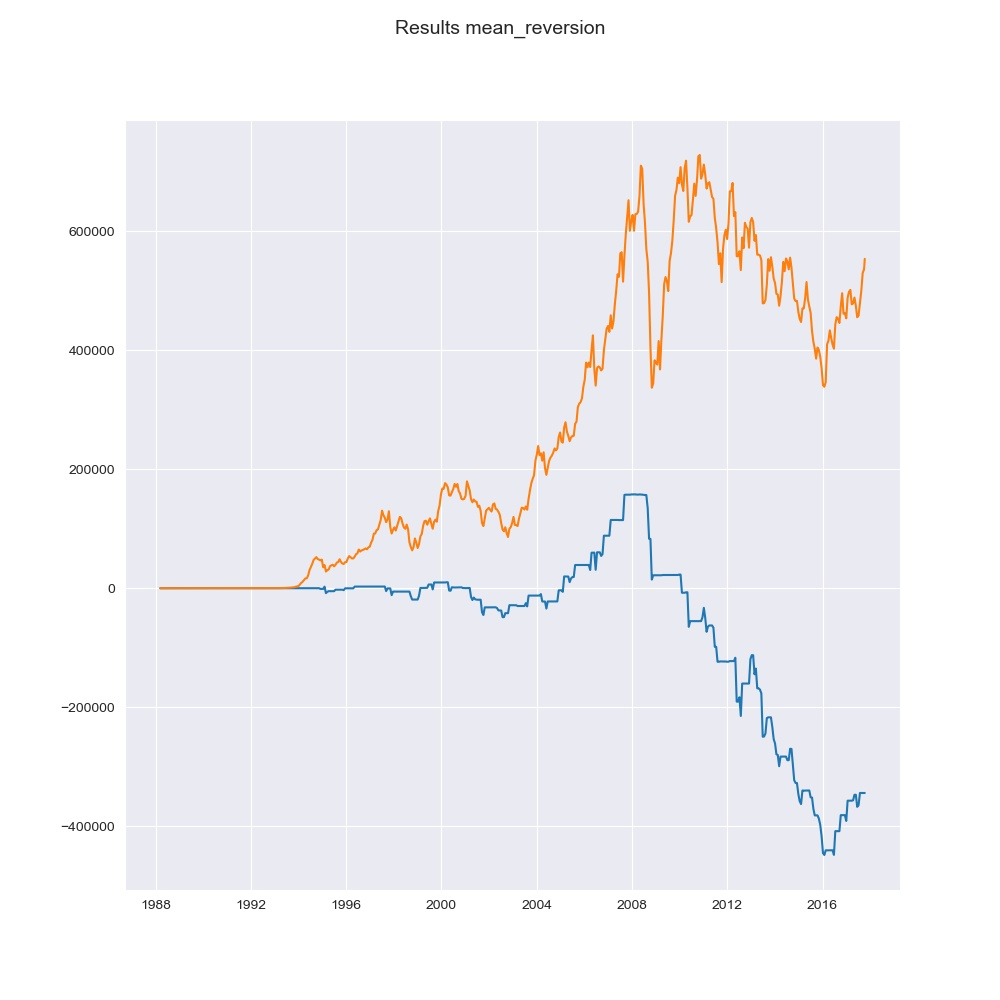
\includegraphics[width=0.48\textwidth]{../results/results_full_ts/mean_reversion_results.jpg}

    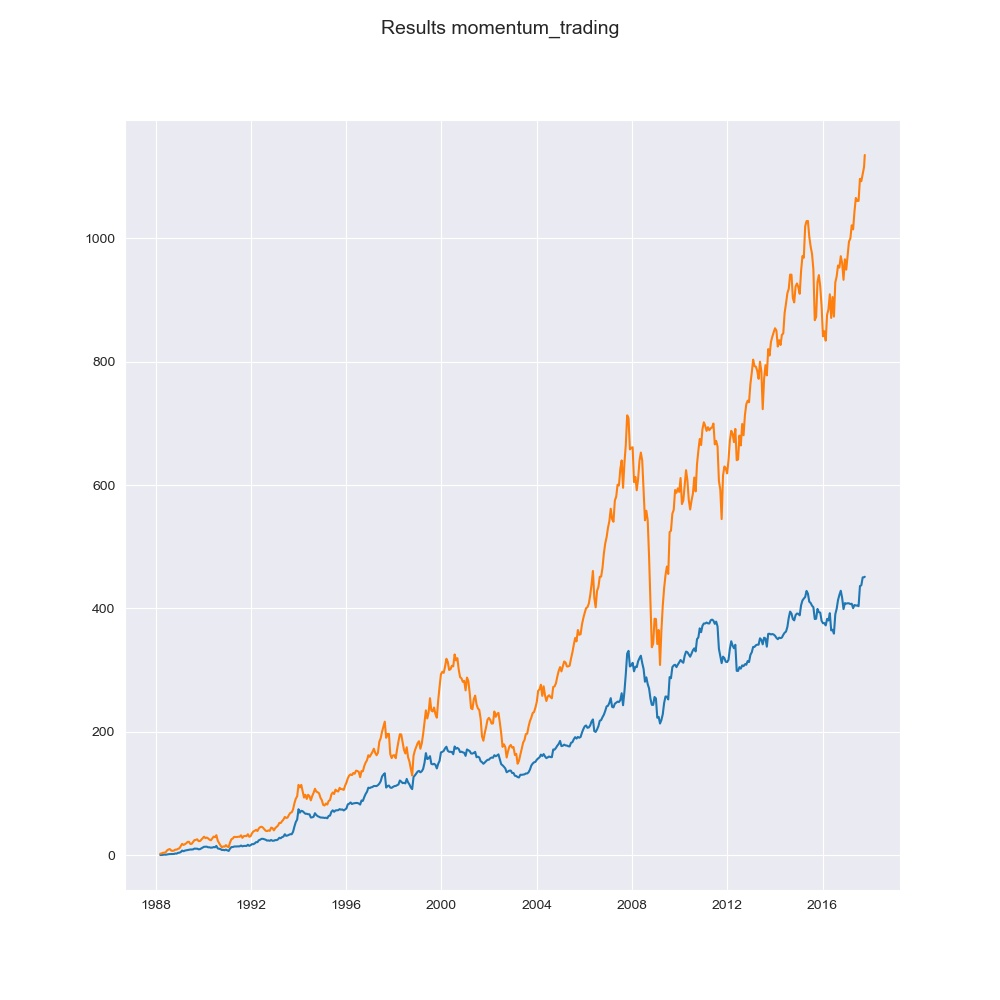
\includegraphics[width=0.48\textwidth]{../results/results_full_ts/outlier_removed_momentum_trading_results.jpg}
    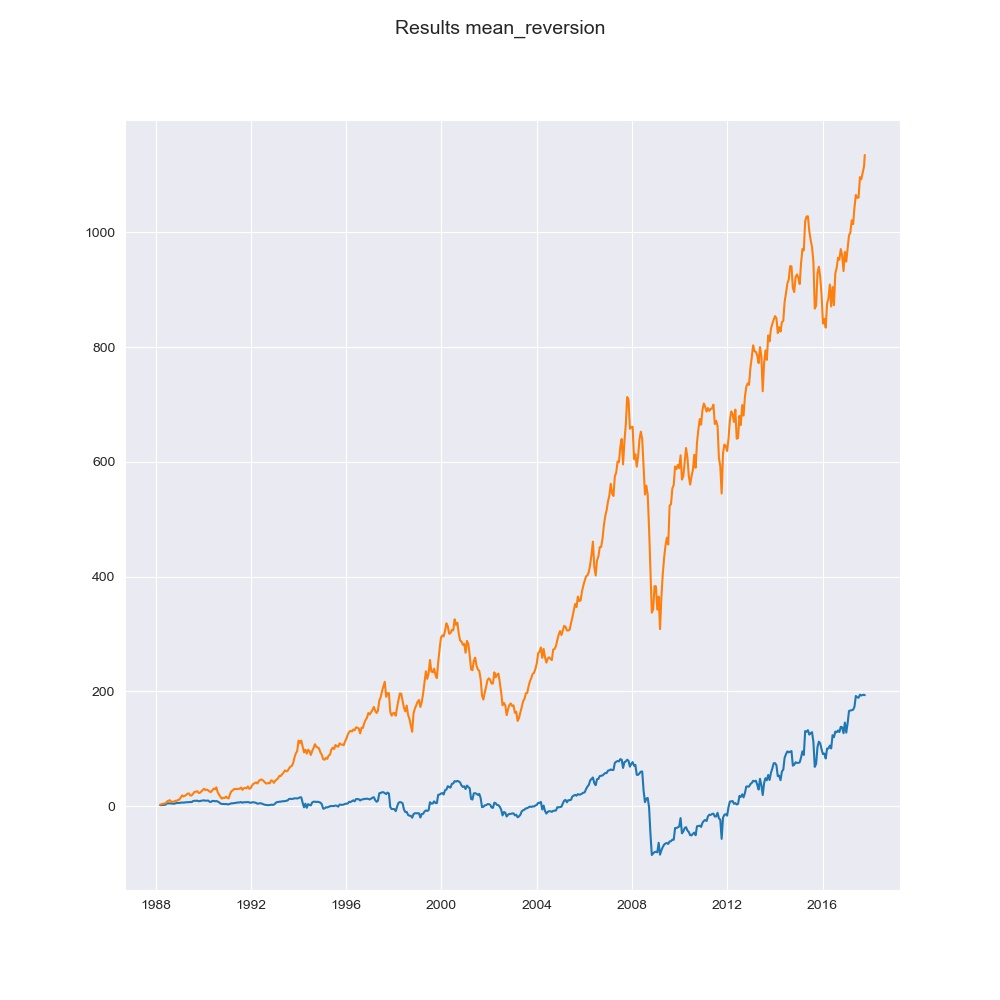
\includegraphics[width=0.48\textwidth]{../results/results_full_ts/outlier_removed_mean_reversion_results.jpg}

    \caption{Results full data set, baseline in orange. Second row: Assets 2 and 25 removed}
    \label{4}
  
\end{figure}{}


\chapter{Code}
the code is available on 

\chapter{Further Considerations}
The trading strategies proposed are in many ways not optimal and not optimized. To a certain extent this is intentional in order to avoid overfitting. But nevertheless there are many parameters to be tuned and ways in which the model could be extended. The trading frequency is one such parameter that could be chosen much shorter or much longer. Especially the time-series based forecasts could work better over a shorter, e.g. daily horizon. This can easily be changed, it just needs more computational power and time. 

\section{Extensions}
Other means of predictions could be used, i.e. vector time series models or machine learning approaches like XGBoost or LightGBM.  

Also the functionality of this backtesting tool could be extended to follow more closely the capabilities of existing backtesting tools. 

% \input{sections/2Performance.tex}
% \input{sections/3Charts.tex}
% \input{sections/4Code.tex}
% \chapter{Reasoning}

The trading strategy I chose is not 

% %\begingroup
% %\renewcommand{\clearpage}{}
% \input{sections/conclusion.tex}
% %\endgroup
% %\printbibliography[heading=bibintoc]
% \clearpage
% \bibliography{bib/mybib}
% \label{bib:mybiblio}
% \clearpage
% \appendix
% \input{sections/Appendix.tex}

% \clearpage
% \input{sections/zdeclaration.tex}


\end{document}



